\documentclass[11pt,twocolumn,twoside]{IEEEtran}
\usepackage{amsmath}
\usepackage[pdftex]{epsfig}
\usepackage{amsfonts}
\usepackage{amssymb}
\usepackage{fancyhdr}
\usepackage{url}
\include{graphicsx}

\pagestyle{fancy}
%\renewcommand{\headrulewidth}{0pt}
\renewcommand{\footrulewidth}{0pt}
\rhead{
\includegraphics[height=0.6in]{cilogo.png}}
\fancyhead[LO]{\sc sci-wms\ldots} % shorter form of title to fit in space
\fancyhead[LE]{\sc Mayer, McKenna, Knee} % author list or et al., to fit in space
\chead{}
\cfoot{}

\begin{document}
\title{\vspace{0.2in}\sc sci-wms:A python-based Web Map Service for Visualizing Geospatial data}

\author{Brandon A. Mayer$^{1,2}$, Brian McKenna$^{2}$, Kelly Knee$^{2}$\thanks{Brown University School Of Engineering$^{1}$, RPS-Applied Science Associates, South Kingston RI$^{2}$, Brandon\_Mayer@brown.edu, BMcKenna@asascience.com, KKnee@asascience.com}}

\maketitle
\thispagestyle{fancy}

\begin{abstract}
This abstract outlines the implementation and technology stack for
visualizing geo-registered coastal forecasting (CF) data using
sci-wms~\cite{wms14}.\footnote{https://github.com/asascience-open/sci-wms}
Specifically, discussing the deployment of sci-wms for visualizing
model data and simulations within the scope of the U.S. IOOS Costal
and Ocean Modeling Testbed cyberinfrastructure as an
extensible visualization tool for qualitativly assessing
society-critical oceanagraphic applications including: forecasts, risk
assessment, model comparison and algorithmic/parameter selection.~\cite{leuttich13}
\end{abstract}

\section{Motivation}
The U.S. IOOS Coastal and Ocean Modeling Testbed (COMT) was formed to
unify otherwise disparate entities in government, academia and
industry to leverage ubiquity of computing hardware and the
proliferation of coastal and oceanagraphic models and data to combat
natural and man-made stressors by accelerating the turnaround from
research and development to operational application of society
critical applications, including forecasting, model comparison, model
skill assessment and algorithmic/parameterization
improvements~\cite{luettich13}. Key to the U.S. IOOS COMT mission is
an extensible tool for quickly visualizing and assessing coastal data.

The OpenGIS Web Map Service (WMS)~\cite{wms14} is a standard
describing a http interface for visualizing geospatial data. Sci-wms
implements the OpenGIS-WMS standard in python using Django as a web
framework and standard cross platform numerical software, Numpy and
Matplotlib~\cite{numpy11, hunter07} for generating rasterized visual
content.

\begin{figure}
  \centering
  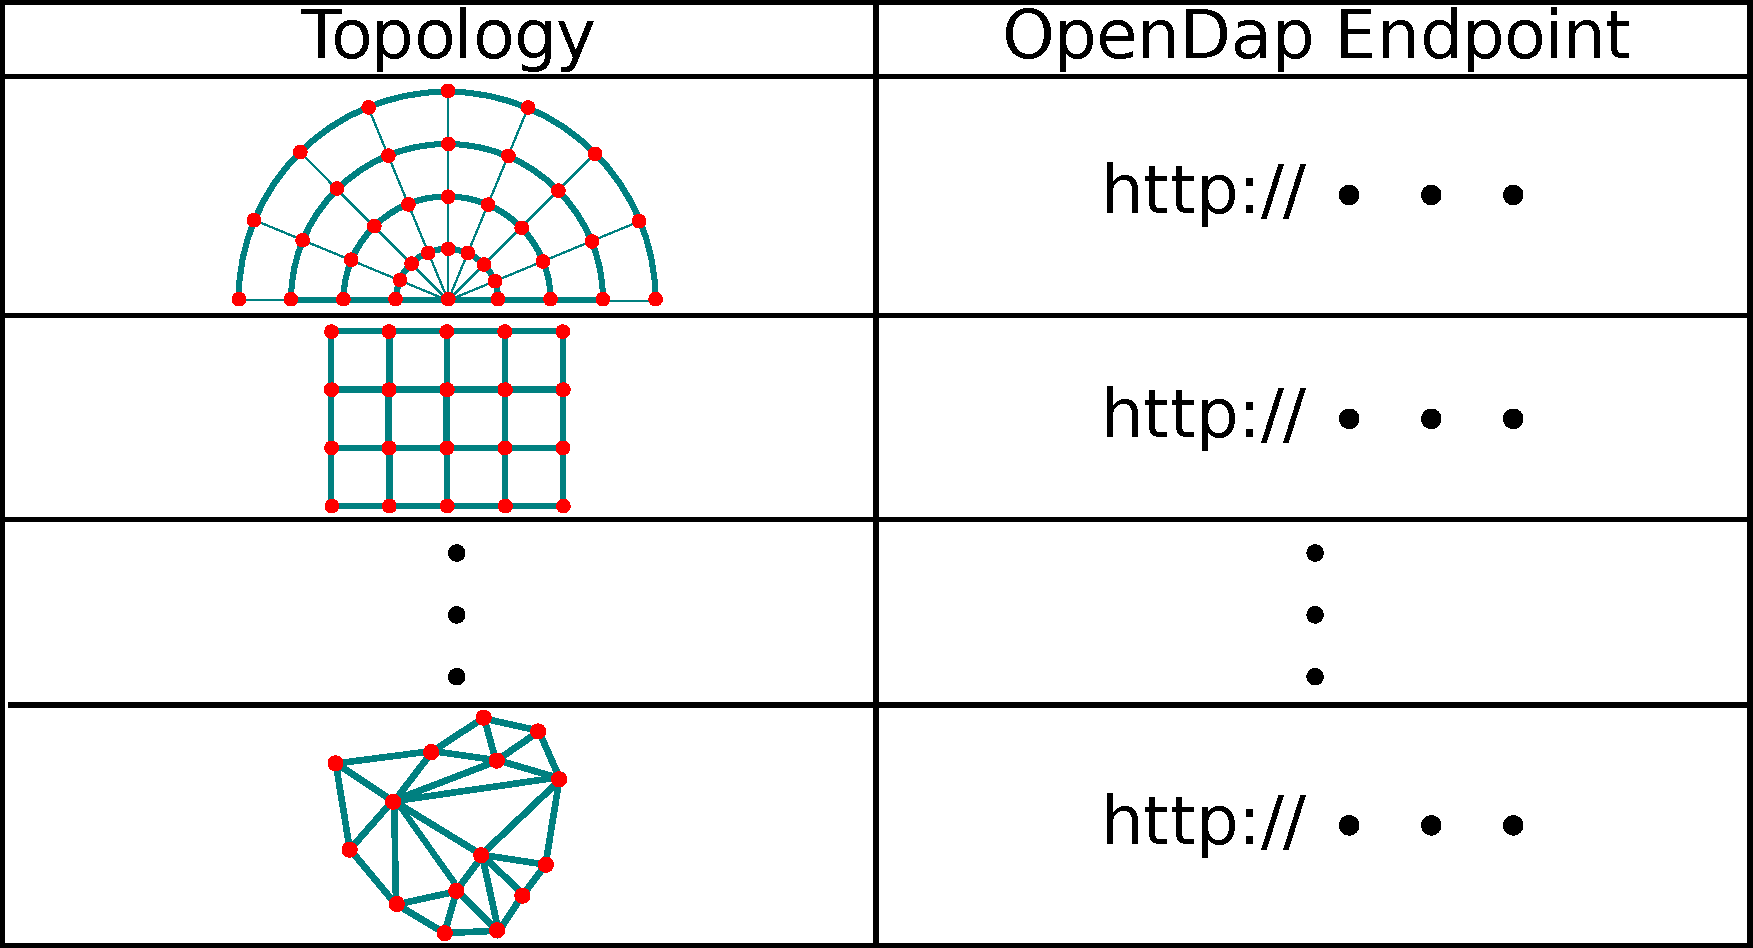
\includegraphics[width=\columnwidth]{./figs/sciwms_db_topology_endpoints.pdf}
  \caption{sci-wms Topology and Endpoint Datastore.}
  \label{fig:sciwms_topology_endpoints}
\end{figure}

sci-wms is a software solution able to visualize meterological
simulations regardless of the underlying methodology by abstracting a
data set into two distinct objects: the simulation topology and
simulation variables. Model topology refers to a geo-referenced set of
geometrical objects which define the positions and connectivity that
variables in the data set may occupy. The types of topologies are just
a numerous as the quantity of standard forecasting models, with some
models able to generate multiple topologies. For example, there are
curvelinear, rectilinear, regular, or unstructured triangular grids
which can be in the planar 2D or volumetric 3D varieties.

\begin{figure}
  \centering
  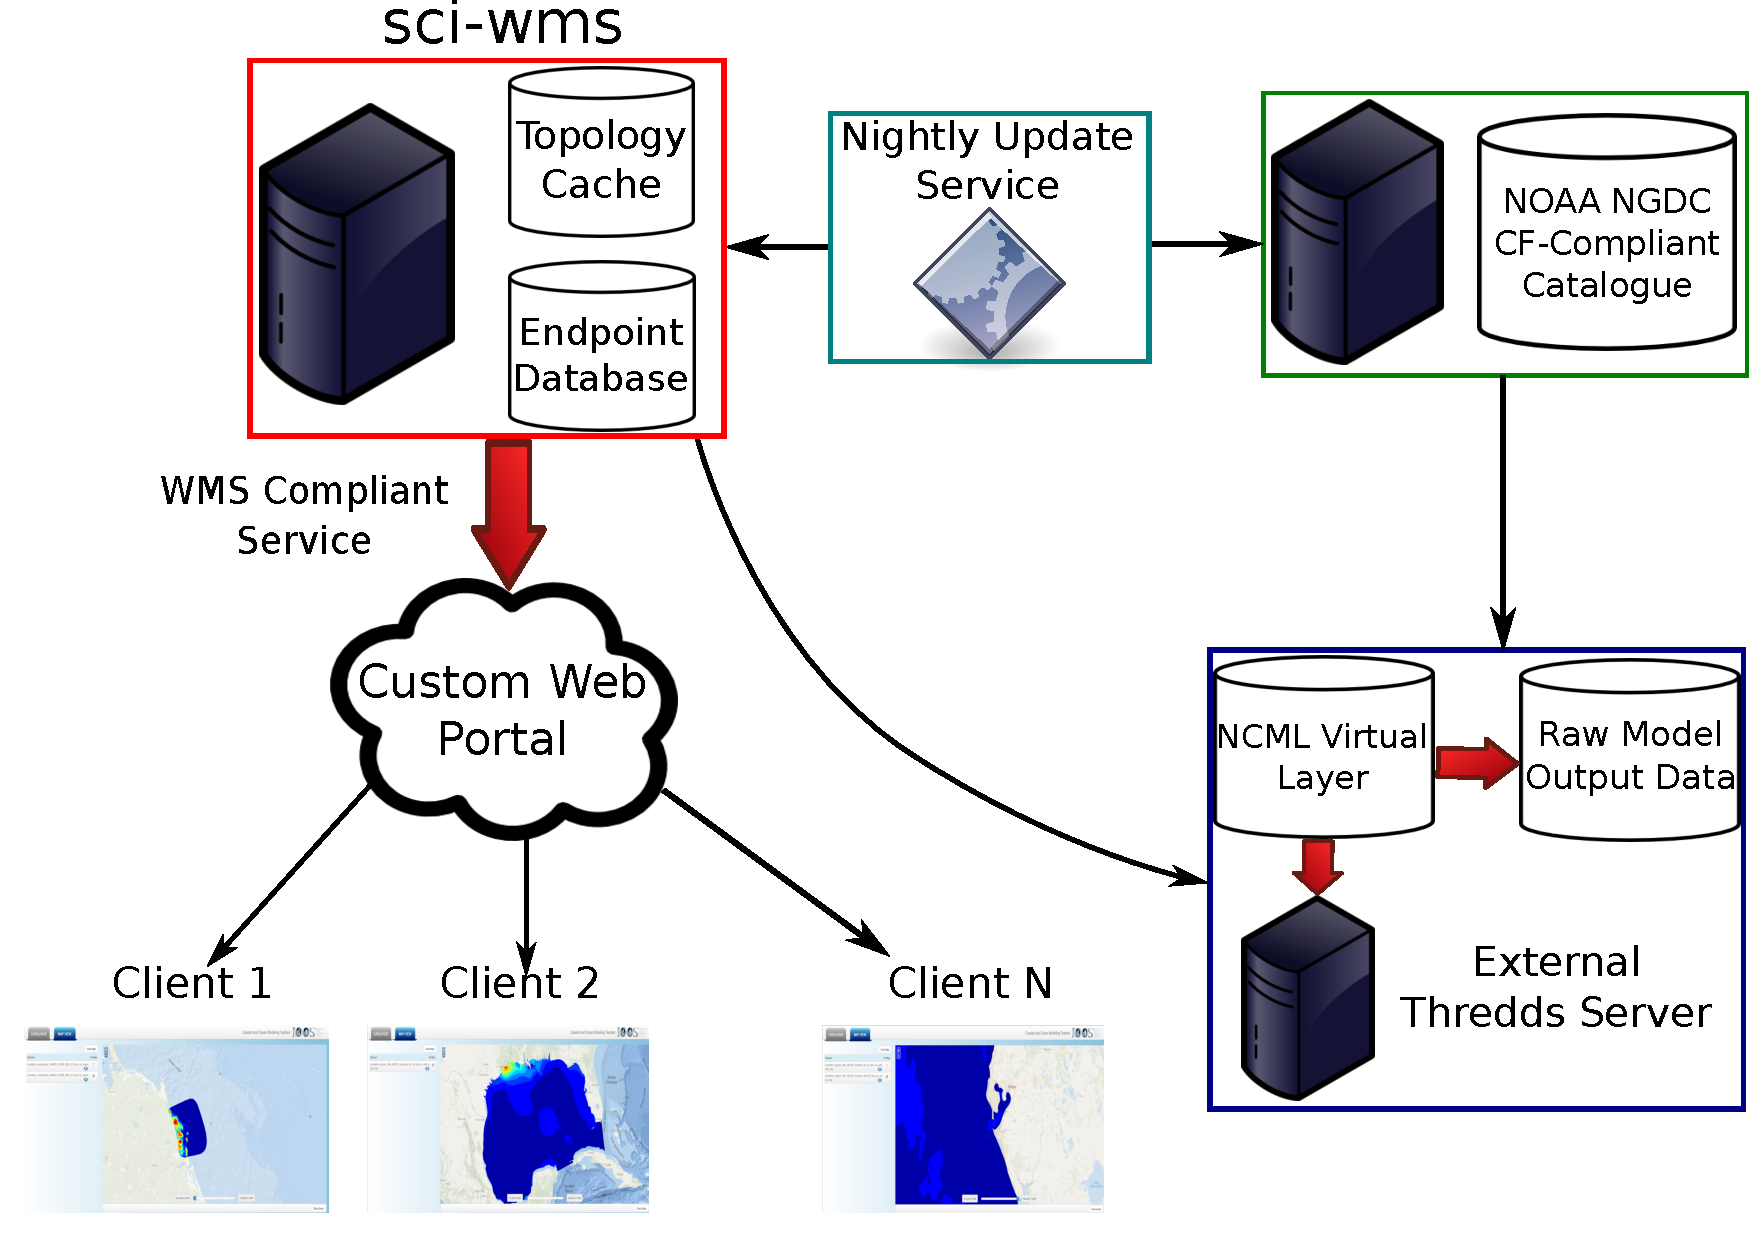
\includegraphics[width=\columnwidth]{./figs/overview.pdf}
  \caption{COMT-SURA deployment of sci-wms for oceanagraphic modeling visualization.}
  \label{fig:overview1}
\end{figure}



\bibliographystyle{ieeetr}
\bibliography{ci_mayer}
%% \bibliography{bibfile,benherzog}

\end{document}
